\documentclass{article}
\title{睡眠とパフォーマンス — 仕組みから改善まで}
\author{TeX 図書館}

\begin{document}

\section{この本の目的と安全性}

ねむることを「回復の時間」だとだけ考えている人がいます。しかし、睡眠は勉強のための道具ではなく、\textbf{勉強そのものの土台}です。勉強した内容を記憶に定着させる。判断の精度を整える。安定した体調を維持する。この 3 つは、\textbf{寝ている間にこそ仕上げられます}。

本章ではまず、本書が扱う範囲と、安全上の注意をまとめておきます。

\subsection{この本は一般的な情報である}

本書は、一般的な知識として睡眠の組み立て方を叙述する本です。\textbf{医療上の助言ではありません}。\textbf{薬や治療については扱いません}。眠り方に関する情報を、\textbf{統計学入門}(効果量・標本数・信頼区間)および \textbf{投資の数学}(半減期・指数減衰)で読み解いていきます。

「医療上の助言ではない」ということを、意味のある形で守るために、次の 3 点を貫きます。

\begin{itemize}
\item 本書は\textbf{あなたの睡眠を診断しません}。眠れないのか眠りすぎるのかという判断を、本書は代行しません。
\item 薬の使い方には触れません。睡眠薬や抗うつ薬、メラトニンの処方は\textbf{医師が}決めるものであり、本書はその代わりになりません。
\item 睡眠時間や眠気スコアは\textbf{目安}であり、\textbf{診断の根拠にはなりません}。
\end{itemize}

\subsection{しっかり眠れないときの相談先}

一晩だけでなく、数週間から数か月続く症状があるときは、本書を読むだけでは足りません。次の症状があれば、\textbf{医療機関で相談してください}。

\begin{itemize}
\item 日中に強い眠りがでて、席で居眠りしてしまう
\item 大きないびきで、同居の人から「寝ているときに息が止まる」と指摘される
\item 脚がむずむずする。就寝前や夜中に悪化する
\item 夜の覚醒が多く、布団が汗ばむ
\item 「眠れない」ことを心配しすぎて、かえって眠れなくなる
\item 十分眠っているのに、日中の眠気が続く
\end{itemize}

これらの多くは\textbf{治療できる症状}です。\textbf{「眠れない自分」を自己判断で慢性的な問題だと決めつける必要はありません}。一方で、改善のための運動が常に有効とは限りません。医療機関では、標準的な検査や治療が用意されています。

\begin{quote}
\textbf{【心構え】}\ 本書は一般的な情報であり、医療上の助言ではありません。\textbf{眠りの問題が続く場合は、医療機関の担当者に相談してください}。\textbf{眠れないこと自体に治療できる原因が見つかることもあります}。本書は、その判断の代わりにはなりません。
\end{quote}

\section{なぜ眠るのか — 回復と思考の準備}

「なんのために眠るのですか」と聞かれると、「疲れたから」と答えるのが普通です。しかし、睡眠には 4 つの役割があります。すべて、眠っている間にはたらきます。

\subsection{物理的な回復}

よく「体の疲れを回復する役割」と言われます。筋肉は睡眠中に壊された細胞を補修します。回復に必要十分な睡眠時間は、おおよそ \textbf{1 日 7〜9 時間}です。

ただし、\textbf{睡眠は体力の回復に必要ですが、体力の回復は睡眠だけでは終わりません}。長時間の回復を求めるなら、栄養と運動も必要です。

\subsection{代謝物のクリアランス}

ここ 10 年で大きく進んだ分野です。\textbf{グリンパティック系}という名称で知られる仕組みが、神経を支える細胞から伸びた血管周りのネットワークを通じて、\textbf{脳内の代謝産物を排出する経路}があることがわかりました。

この経路は徐波睡眠(第 4 節)のときに特に活発に働きます。\textbf{「眠ると老廃物が下がる」}という表現は単純化されているため、\textbf{「排出されるものもある」}と読み替えてください。

\begin{quote}
\textbf{【補足】}\ グリンパティック系という名称は、神経を支える細胞に由来します。医療機関でよく出てくる専門用語ですが、本書ではここ以上に立ち止まりません。数式で扱う対象ではありません。
\end{quote}

\subsection{記憶の定着}

これが第 12 節の主題です。記憶には 2 層あります。\textbf{海馬}と呼ばれる脳の部位が一時保管する短期記憶と、大脳皮質に広く分散している長期記憶です。一晩の睡眠のあいだに、後者が前者から\textbf{転写・再構築}されます。

つまり、記憶は受動的な現象ではありません。\textbf{頭で考え理解了だけでは定着しない}——使用した時間と眠った時間の組み合わせで、定着の質が決まります。\textbf{寝た後に思い出せるかどうか}が、記憶の出来栄えを決めます。

\subsection{免疫と回復力}

睡眠不足は免疫を下げます。心筋血管の疾患との関連を調べた観察研究のうち、1980 年代から 90 年代の野球選手の研究では、睡眠 6 時間未満の選手では、血中の炎症を示す蛋白が高い傾向が報告されました。\textbf{この関係は方向としては明確ですが、サイズを断定するほど精密ではありません}。

逆に、睡眠不足の状態からでも、感染時に発熱する能力は回復します。\textbf{「運動すると風邪を引く」のは、睡眠不足の時により強く出ます}。このため睡眠は、感染症対策の投資と見なせる場合もあります。

\begin{quote}
\textbf{【演習】}\ 睡眠の 4 つの役割(回復・代謝物のクリアランス・記憶の定着・免疫)から、自分の生活で一番影響が大きいと感じる役割を 1 つ選び、その役割を睡眠で改善する具体的な方法を 1 つ書け。
\end{quote}

\textbf{解答の指針:}\ 例として「記憶の定着」を選んだ場合、答えは次の 3 通りに分解できる。\textbf{① 記憶したいものを寝る直前に総復習する}。\textbf{② 寝室を静か・暗い・涼しくする}。\textbf{③ 翌朝に仮説を検証する}。どの役割でも「その役割が働く条件」は本文に書かれている。\textbf{役割を 1 つ決めるのではなく、条件を 3 つに分解する}と行動になりやすい。「記憶の定着」は『統計学入門』の信頼区間と組み合わせると、効果がどれだけかも報告できる。

\section{2 つのプロセス — 眠気は 2 つの合力で生まれる}

眠気は 1 つの原因では決まりません。\textbf{2 つのプロセスが競合して作用している}とするモデルが、2 プロセスモデルです。1970 年代に提示され、改良を重ねた、今でも中心的な枠組みです。

\subsection{プロセス S — 睡眠圧}

眠気の源になるのは、起きて いるあいだに積み上がる量です。寝ているあいだに分解され、起きているあいだに蓄積します。\textbf{覚醒している時間が長くなるほど、寝る必要は増す}——これがプロセス S です。

科学的には\textbf{アデノシン}という物質が関わっています。起きているとアデノシンが蓄積し、脳の受容体に結びついて眠気を生みます。\textbf{アデノシンは眠ることで消え}、朝には正常な状態に戻ります。したがって \textbf{昼寝をすれば眠気は一時的に下がる}。夜の睡眠は夜の仕事です。

\subsection{プロセス C — 覚醒推進}

もう 1 つは\textbf{覚醒を押し上げる}プロセスです。これは概日リズム(体内時計)から来ます。第 5 節で詳しく扱います。

\textbf{「昼寝を長くすると、その夜は眠りにくくなる」}のは、プロセス S ではなく \textbf{プロセス C} があるために起きます。昼寝でアデノシン(プロセス S)は下がっても、\textbf{体内時計は「まだ昼だ」と認識している}。短時間の昼寝は安全ですが、1 時間以上は就寝時刻を後ろに押し、\textbf{その夜の入眠を遅くする}。

\begin{figure}[h]
\centering
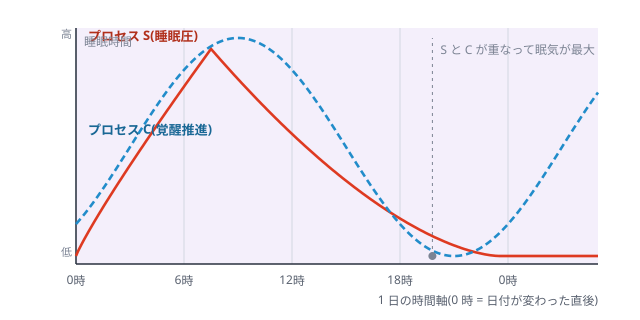
\includegraphics[width=0.85\textwidth]{figures/two-process.svg}
\caption{プロセス S と プロセス C の 1 日の動き。S は起きているあいだに上昇し、寝ると下がる。C は約 24 時間周期で振動する。深夜において両者が重なるとき、眠気が最も強くなる。}
\end{figure}

\subsection{2 プロセスが説明できること}

2 プロセスモデルは日常のあちこちを説明できます。

\begin{enumerate}
\item \textbf{午後の眠気}: 午後は S が高まりつつも、C は一度大きく落ちます。\textbf{午後の眠気は体内時計の落ち込み}であり、\textbf{弱さの証拠ではありません}。
\item \textbf{「今日は早寝できない」}: S の値ではなく、\textbf{C が高い}から眠れない場合。カフェインも C を強めます。
\item \textbf{寝正月}: 寝正月という表現は、実際の睡眠不足とは別です。\textbf{眠気はないのに夜に眠れない}状態です。第 11 節で扱います。
\end{enumerate}

\begin{quote}
\textbf{【定義:2 プロセスモデル】}\ 眠気(睡眠の意思強度)は、(1) 覚醒している長さに比例して積み上がる睡眠圧(プロセス S)と、(2) 約 24 時間周期で振動する覚醒推進(プロセス C)の \textbf{2 つの合力}として説明する枠組みです。
\end{quote}

\begin{quote}
\textbf{【演習】}\ ある人が「昨日 4 時間しか寝なかったのに、昨日はよく眠れたので問題ない」と言う。この発言は、プロセス S による説明とプロセス C による説明のどちらで整合するか。また、今日午後 3 時に 20 分寝た場合、その夜の入眠にどう影響する可能性が高いか言え。
\end{quote}

\textbf{解答の指針:}\ 睡眠時間が短いのに眠れたのは、眠気という合力が一時的に低かったからです。プロセス S は上昇しますが、\textbf{眠ったという事実が S を下げる}ので、その夜の回復自体には問題がありません。問題は翌日に持ち越されます。一方、20 分の昼寝はプロセス S を少し下げますが、アデノシンは完全には消えません。\textbf{昼寝で下げた眠気を夜に持ち越すと、その夜の睡眠が浅くなる}。「昼寝は夜の睡眠を壊さない」ということの意味は、ここまでが正確な範囲です。

\section{睡眠段階 — 一晩を構成する部品}

一晩の睡眠は、単なる「眠っている時間」ではなく、\textbf{性質の異なる段階の繰り返し}です。脳波のパターンで区分します。\textbf{この区別は「よく眠った」を意味のある言葉にするための道具}になります。

\subsection{N1・N2・N3 — 非 REM 睡眠}

\begin{quote}
\textbf{【定義】}\ \textbf{非 REM 睡眠}は、目が閉じていても脳が活動を続ける段階です。3 つの深さの段階に分けます。
\end{quote}

\begin{center}
\begin{tabular}{|l|c|l|}
\hline
段階 & 全体に占める割合 & 特徴 \\
\hline
N1 & 2〜5\% & 入眠の直前。意識はまだあり、眠りは浅い \\
N2 & 45〜55\% & 睡眠の本体。脳波に睡眠スパイクが混じるが回復は進む \\
N3 & 13〜23\% & 徐波睡眠。\(1\,\mathrm{Hz}\) 以下のゆっくりした波で、回復が最も進む段階 \\
\hline
\end{tabular}
\end{center}

割合は目安です。\textbf{年齢が上がるほど N3 の割合は減少し、N2 と覚醒が増えます}。若者は一晩のうち約 15〜25\% を N3 に使うため、一晩 1 時間の N3 不足は大きな損失です。

\subsection{REM 睡眠}

\textbf{Rapid Eye Movement(速い眼球運動)の睡眠}が略称です。他の眠り，下列 のような特徴を持ちます。

\begin{itemize}
\item 脳は覚醒状態に近い活動をする(このため夢を見やすい)
\item 随意筋がほとんど動かない(\textbf{骨格筋の弛緩}、ただし呼吸に関わる筋は動く)
\item 一晩のうち 1 番目と 2 番目のサイクルに集中して出現する
\item 後半になるほど停滞して長くなる
\end{itemize}

\begin{quote}
\textbf{【例:REM と記憶の矛盾】}\ REM 睡眠で学んだ内容はよく出ます。\textbf{REM は記憶の単純な保存ではなく、再構築という役割}を演じます。REM を完全に削った場合、情緒や手続き記憶に影響がある、と報告されています(ただし研究ごとに方法は異なります)。
\end{quote}

\subsection{サイクルという考え方}

一晩の睡眠は、深い谷と山が交互に現れる形状になります。\textbf{一つの山と谷を「サイクル」と呼びます}。成熟した成人の場合、\textbf{一晩で 4〜6 サイクル}です。サイクルごとに REM の長さと深い睡眠の長さが変化するので、「サイクル」と「段階」を混ぜないことが大切です。

\begin{figure}[h]
\centering
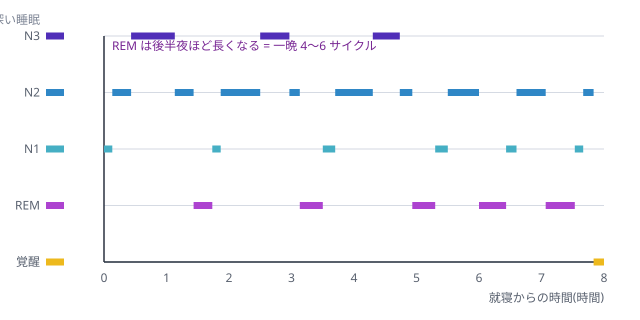
\includegraphics[width=0.85\textwidth]{figures/hypnogram.svg}
\caption{典型的な一晩の睡眠図。横軸は就寝からの時間、縦軸は睡眠段階。REM は最初のサイクルでは短く、後半夜ほど長くなる。}
\end{figure}

\subsection{「90 分サイクル」という言い回スを信用しない}

「1 サイクルは 90 分。これは教科書の定数」——と信じている人が多いです。\textbf{ここが最も誤りやすいポイントです}。

睡眠の 1 サイクルは\textbf{人によって幅が大きく異なる}うえ、\textbf{その夜のなかでも変動します}。90 分ちょうどと仮定してアラームを鳴らすのは、\textbf{逆効果}です。\textbf{90 分は平均値にすぎません}。

\begin{quote}
\textbf{【演習】}\ 90 分周期という言い回スを根拠に、22 時に就寝して翌朝 6 時に起きることを計画する人がいます。1 サイクルを 90 分と仮定するといくつのサイクルになるか計算し、その仮定が実際にどれほど危険であるかを、サイクル数と睡眠の質の関係から説明せよ。
\end{quote}

\textbf{解答の指針:}\ 22 時から 6 時までで 480 分、\(480 / 90 \approx 5.3\)。この計算で「5〜6 サイクル」と概算することは正しい。\textbf{危険なのは「90 分目」で起きること}。サイクルの幅は 70〜120 分と幅があるため、90 分ちょうどに出た場所では \textbf{睡眠の最も深い部分をしたまま起こす}ことになる。\textbf{起きる時間の設計はサイクルと関係なく、「何時間眠るか」だけで決めるのが正解}です。

\section{概日リズム — 体内時計というリズム}

24 時間周期で繰り返される体のリズムを\textbf{概日リズム}(circadian rhythm)と呼ばします。\textbf{眠りのタイミングを決めるのはこの時計}です。

\subsection{SCN — 視交叉上核}

体内時計の中心は\textbf{視交叉上核}(SCN)と呼ばれる脳の部位です。目のすぐ裏、視神経の交差する場所のすぐ上にあります。\textbf{約 2 万個のニューロン}からなる小さな核ですが、ここが「主時計」です。

\begin{quote}
\textbf{【補足】}\ 「朝起きて、朝の光を受けると体内時計が調整される」——第 9 節で使う最重要の手法です。目の裏には青色光に最もよく反応する視細胞があり、\textbf{その細胞が青色(波長 460〜480 nm 前後)を認識して SCN を動かします}。
\end{quote}

\subsection{光とメラトニン}

光が SCN を刺激すると、\textbf{松果体でメラトニンの分泌が抑えられます}。逆に暗くなると、\textbf{「暗くなった」ことを脳に知らせる物質}が出はじめます。\textbf{メラトニンは眠りを招く物質ではなく、「暗い」ことを知らせる物質です}。

重要なのは、\textbf{この「暗い」合図は消灯時刻だけで決まらない}ことです。\textbf{寝つきが悪い人に「早く消灯しなさい」と勧めるのは、本質的に逆効果}。\textbf{体内時計を整えるのは消灯時刻ではなく起床時刻}。第 7 節の重要な根拠です。

\subsection{体内時計をずらす}

体内時計の周期は、24 時間ちょうどではなく、およそ 24.2 時間だとされます。\textbf{毎日同じ時刻に起きることで，毎日のズレを打ち消す}必要があります。

\begin{quote}
\textbf{【定義:光と体内時計の位相】}\ \textbf{光(特に青色光)を暴露した時刻が体内時計の位相を決める}。朝の光は体内時計を早める方向に、夕方の光は遅らせる方向に作用する。
\end{quote}

\begin{quote}
\textbf{【演習】}\ 体内時計を早める方向にずらすために、その日のうちで最もよく効く時刻はいつか。答えと、その理由を光と起床の関係を踏まえて述べよ。
\end{quote}

\textbf{解答の指針:}\ 答えは\textbf{「起きた直後の朝」}です。\textbf{体内時計を早めるなら、午後ではなく朝に強い光を当てる}。逆に遅らせるなら夕方に強い光を当てる。\textbf{「夜更かしを直すには寝る時間を早める」だけでは不十分}で、\textbf{朝の光が鍵になる}。第 9 節の最初の項目が、具体的な操作です。

\section{なぜ、たまに悪い夜を気にしなくてよいのか}

「一晩だけ 2 時間しか寝なかった。明日は最悪だ」——この恐怖(睡眠不安)を解きほぐすのに、科学は明確な答えを出しています。

\subsection{睡眠負債はゆっくり回復する}

寝不足を睡眠負債と呼びます。\textbf{睡眠負債は一晩でまとめて返す必要がありません}。\textbf{回復は数晩にわたって段階的に進行します}。図のように、0 夜目だけ 5 時間(3 時間不足)とした場合、1 夜目は通常より少し長く寝て回復の過程を始めます。

\begin{figure}[h]
\centering
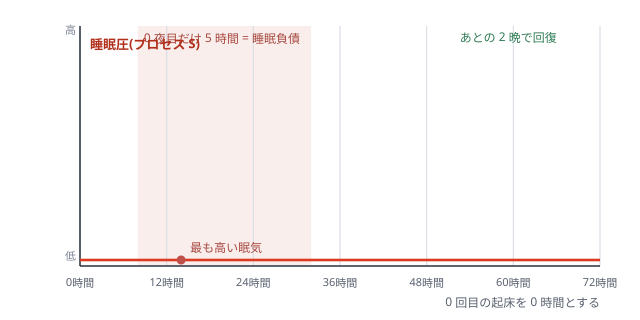
\includegraphics[width=0.85\textwidth]{figures/sleep-debt.svg}
\caption{睡眠負債の回復。0 夜目だけ 5 時間に短縮した場合を例に、回復が 2 晩で大体終わる様子を示す。1 晩ですべてを元に戻す必要はない。}
\end{figure}

\subsection{ただし、回復に頼れるのは 2 晩まで}

大きな睡眠負債は回復に 2 晩ほどかかるのが定例です。\textbf{つまり、1 晩だけの不足なら 2 晩で回復できる}。しかし\textbf{週に 6 日 4 時間 しか眠らない場合、負債は蓄積する一方}で、回復は追いつきません。

\subsection{悪い夜を長時間寝て取り戻そうとはしない}

悪い夜のあとに\textbf{昼寝で一気に取り戻そうとする}戦略も逆効果です。昼寝を長くすると、
\begin{enumerate}
\item 体内時計がずれ、次の夜に入れない。
\item その夜の回復機会(N3 と REM)を削る。
\item 悪化する悪循環が続く。
\end{enumerate}

\textbf{正解は「悪い夜の翌朝には、いつもどおり(可能なら少し早く)の時刻に起きる」}ことです。こうすれば次の夜に自然に入れできます。

\begin{quote}
\textbf{【演習】}\ 試験が終わった翌日、午前 0 時に 6 時間眠った。翌朝 14 時に起きる計画である。\textbf{この計画の問題点}を 2 プロセスモデルの枠組みで評価し、よりよい代替案を 1 つ示せ。
\end{quote}

\textbf{解答の指針:}\ 「翌朝 14 時起床」そのものが体内時計を大きく乱す。また就寝時刻が遅いと、起床時刻も遅れるため、次の夜の睡眠が短くなる。代替案は 2 つ。\textbf{(1) 起床時刻を平时どおりに固定して 2 日目からやり直す}——0 夜目の睡眠負債は 2 晩で回復します。\textbf{(2) 1 日目は多少きついが、平时どおりに寝る}。\textbf{「取り戻す」より「乱さない」ことのほうが、長期の成績はよい}。

\section{起きる時間の設計 — 一番効く「一行」}

多くの人は「眠る暇がない」と考えます。しかし、\textbf{実際に足りないのは「眠る暇」ではなく「起きる時間の設計」}です。別の言い方すると、\textbf{総睡眠時間は「起きる時間」によって決まる}。

\subsection{総睡眠時間 = 起きる時間 − 必要睡眠時間}

ここが本書で一番使う式です。

\begin{quote}
\textbf{【定義:総睡眠時間の設計式】}\ \textbf{総睡眠時間 ＝ 起きる時間 − 必要睡眠時間}。\textbf{起きる時間が決まれば、眠れる総量は自動的に決まる}。決めるべきは「早起きするか」ではなく、\textbf{「何時に起きるか」だけ}です。
\end{quote}

たとえば、必要睡眠時間を 7.5 時間とする成人が 7 時に起きると決めた場合、\textbf{入眠までに 30 分を余裕として取ると、就寝時刻は 22 時}です。「23 時に寝れない」ことは問題ではなく、\textbf{「起きている時間が長すぎる」}ことが問題でした。

\subsection{「起きる時間」の方が重要な理由}

前述のとおり、\textbf{体内時計に影響するのは「消灯時刻」より「起床時刻」}です。あなたが受け取る光のなかで最も強いのは、\textbf{「朝、目が覚めた直後の光」}。まずここだけを揃えれば、体内時計は半分は追いつきます。

習慣上は就寝時刻を決めるほうが楽ですが、\textbf{実際に効くのは起床時刻を固定すること}。前者はあとの計算結果、後者は最初に決める数字です。

\subsection{カフェインの半減期}

\textbf{カフェインの半減期は約 5.5 時間}です。すなわち、\textbf{今飲んだカフェインの一半は、5.5 時間後にはまだ体内にある}。継続的に飲む場合、\textbf{1 日のうち半分の時間は血中濃度が半分以上のまま}です。

\begin{quote}
\textbf{【例】}\ ある事務員が 9 時と 14 時にそれぞれコーヒー 2 杯を飲むとする。\textbf{重要なのは「何時に飲んだか」であって、「何杯飲んだか」ではない}。濃度は
\[ C(t) = C_0 e^{-kt}, \qquad k = \frac{\ln 2}{t_{1/2}} \]
という指数関数の減衰で表せる。\textbf{投資の数学}で扱った減衰と同じ形である。
\end{quote}

\begin{figure}[h]
\centering
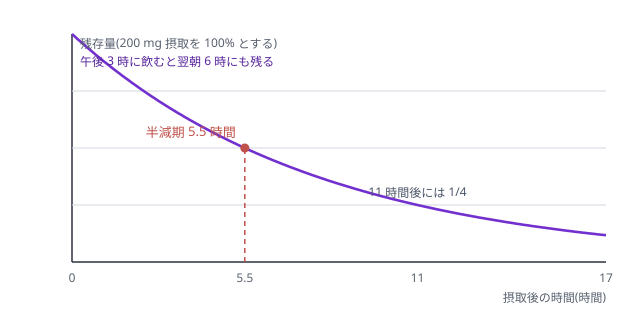
\includegraphics[width=0.8\textwidth]{figures/caffeine.svg}
\caption{カフェインの減衰。半減期が 5.5 時間であるため、午後 3 時に飲んだ分は翌朝 6 時(15 時間後)でもおよそ 1/8 が残る。}
\end{figure}

\begin{quote}
\textbf{【演習】}\ 半減期 5.5 時間のカフェイン 200 mg を\textbf{午後 3 時に飲んだ}。\textbf{午前 9 時(18 時間後)の残存量}を求めよ。
\end{quote}

\textbf{解答の指針:}\ 半減期が 5.5 時間なので、18 時間は \(18 / 5.5 \approx 3.27\) 個の半減期を経過する。
\[ C(18) = 200 \times \left(\tfrac{1}{2}\right)^{18/5.5} \approx 200 \times 0.104 \approx 20.8\ \text{mg} \]
となる。\textbf{「夜中に飲まなかったから」だけでは翌朝は落ち着かない}理由がこれです。\textbf{「午後 3 時以降に飲まない」というルールは、この計算から自然に導かれる}。

\begin{quote}
\textbf{【補足】}\ 半減期の式は、\textbf{「濃度は最初の量から減る割合が一定}、つまり\textbf{同じ割合で減り続ける}」ことを意味します。\textbf{投資の数学}における期待値計算と同じく、\textbf{足し算ではなく掛け算で効いてくる}ため、\textbf{一度に摂取するより継続して少しずつ飲むほうが血中濃度が下がりにくい}。
\end{quote}

\section{カフェインとアルコールの罠}

性能を下げる 2 つの代表的な物質についてまとめます。\textbf{「悪者」扱いではなく、「用量と時間を設計する材料」}として扱います。

\subsection{カフェイン — アデノシン受容体をブロックする}

カフェインは脳に直接作用して覚醒させるのではありません。\textbf{アデノシンの受容体に結合して、アデノシンの眠りを促す信号を塞ぐ}ことが本質です。

\begin{quote}
\textbf{【補足】}\ 「カフェインで REM を削る」という言い方は正確ではない。カフェインは REM 睡眠自体を直接抑制する力は小さい。\textbf{「そのぶん眠気が減ったと感じ、眠り始めない」}結果、\textbf{総睡眠量が減る}。つまり、\textbf{悪影響は「REM の直接的な減少」ではなく「眠りの機会と総量の減少」}として現れます。
\end{quote}

\subsection{午後 3 時という締め切り}

\textbf{午後 3 時以降のカフェインを避ける}——これが単純なルールです。\textbf{理由は半減期 5.5 時間}。午後 3 時に 200 mg を飲むと半夜に半分以上が残り、午前 9 時には 1/8 程度が残っている。\textbf{その量でも体内に影響を及ぼしうる}からです。\textbf{「午後 3 時」 という具体的な時刻は厳密な医学的ガイドラインではありませんが、統計的にも安定して効果が出ると考えられます}。

\begin{quote}
\textbf{【例】}\ 午後 3 時に 200 mg を飲んだ人が、午後 11 時に眠る場合。11 時から 3 時までが 8 時間。残存量は
\[ 200 \times \left(\tfrac{1}{2}\right)^{8/5.5} \approx 200 \times 0.364 \approx 73\ \text{mg} \]
となる。\textbf{まだ半分以上が残っている}。\textbf{入眠に 30 分以上かかるのは不自然}であり、寝たあとその 8 時間を実際に眠れていなければ、\textbf{翌朝にカフェインの残りが「空腹」のように効いてくる}。
\end{quote}

\subsection{アルコールの仮眠り問題}

アルコールは一見「寝つきを早める」ように見えます。実際には入眠を早める報告もあります。\textbf{しかし深刻な副作用が 2 つあります}。

\begin{enumerate}
\item \textbf{REM 睡眠の抑制}: アルコールは REM 睡眠を著しく削ります。記憶の定着や情緒の処理に影響を及ぼします。
\item \textbf{後半夜の断片化}: 代謝が進むにつれ、後半夜ほど覚醒が増えます。\textbf{寝る時刻への効果は大きく、質への効果は逆向き}。この現象を\textbf{反動}(rebound)と呼びます。
\end{enumerate}

\begin{quote}
\textbf{【補足】}\ \textbf{反動}とは、\textbf{REM 睡眠を一度抑制した後、その反動で REM を通常より多く出す現象}です。\textbf{「泥酔でぐっすり寝て、翌日疲れが残った」}の正体は、この\textbf{後半夜の目覚め}です。\textbf{翌朝がすっきりしないのは、深い睡眠が取れている証拠ではなく、後半夜が断片化しているため}です。
\end{quote}

\begin{quote}
\textbf{【演習】}\ 血中のアルコール濃度が時間とともに指数関数で減衰すると仮定する。半減期が 7 時間と仮定したとき、\textbf{22 時に晩餐を終え、そのなかでやや多い量のアルコールを摂取した}場合、\textbf{翌朝 7 時(9 時間後)に残る濃度は摂取濃度の何\%になるか}。\textbf{夜間の覚醒との関係}を述べよ。
\end{quote}

\textbf{解答の指針:}\ 9 時間は半減期 7 時間の約 1.29 倍だから、残る濃度は \textbf{約 42\%}である(概算、\(100 \times (1/2)^{9/7} \approx 41\%\))。\textbf{「眠れる時間」が入眠から 4〜5 時間後につづく}ことが原因です。\textbf{入眠は早いが、途中の質が崩れる}——\textbf{「よく眠った」と感じない理由}になります。

\section{行動の工夫 — 環境と習慣の設計}
睡眠を変える方法を、根拠が強い順に並べます。\textbf{まず、環境から直す}を優先します。

\subsection{朝の光 — 10 分、外で}

\textbf{朝、目が覚めてから 10 分以内に、屋外で 10 分}。これで変化するのは「光」です。\textbf{光量の目安}として、屋内照明はおよそ 100〜500 ルクス、\textbf{屋外は 10 万ルクス以上}です。\textbf{200 倍以上の差}があります。

一日をすべて室内で過ごすと、\textbf{体内時計にとっては事実上「暗」のまま}です。

\begin{quote}
\textbf{【演習】}\ 冬の東京で朝 7 時に起き、1 週間朝の 10 分を室内で過ごすことにした。\textbf{この選択が体内時計に与える影響}を、光量の尺度で定量的に論じよ。
\end{quote}

\textbf{解答の指針:}\ 室内光はおよそ 100〜500 ルクス、屋外は 10 万ルクス以上——\textbf{200 倍以上の差}。この差が大きいため、\textbf{「外に出る」という行動そのものが光量を大きく変えます}。\textbf{朝の光を 10 分浴びると、体内時計を早める方向に動かします}。室内では 500 ルクスにも届かないことも多く、効果は得にくい。

\subsection{夕方の光 — 暖色にする、明るさを落とす}

朝は光、夕方は暗くする。\textbf{これが対称}。
朝は光、夕方は暗くする。\textbf{これが対称}。就寝の 1 つか 2 時間前から、照明の明るさを 3 割落とす。色温度を下げて、暖色の灯りに変える。

\subsection{画面 — 就寝前の扱い}

画面から出る青い光は抑制したい成分です。\textbf{ただし、原因は画面そのものではありません}。\textbf{「青い光を出している時間と量」}のほうが問題です。
そのため 2 段階で扱います。\textbf{第一に、寝る 1 時間前は画面を見ない時間をつくる}。\textbf{第二に、画面の色を暗くする}。第一が本筋で、第二は補助です。

\subsection{温度}

\textbf{寝床に入っている間は体温が下がります}。\textbf{周囲的温度が高いと体は冷えず、入眠しにくくなります}。一般には、\textbf{18〜20 度が目安}です。

ただし個人差があります。\textbf{18 度は人によって寒すぎます}。\textbf{適正温度は国や季節、個人の状態によって変わる}ので、\textbf{「暑かったら少し下げ、寒かったら少し上げる」を 3 晩試す}のが確実です。

\section{ナップの設計 — 短い眠りを使い切る}

昼寝は悪いことではありません。\textbf{適切に設計すれば 1 日の性能を上げる手段}です。\textbf{「何分眠るか」がすべて}を決める。

\subsection{20 分と 90 分の違い}

\begin{quote}
\textbf{【定義:20 分の昼寝の位置づけ】}\ 20 分は、\textbf{「深い睡眠に入れるか入れないか」の境界}にあたります。\textbf{睡眠酔いの副作用が最小}で済みます。
\end{quote}

90 分は 1 サイクルまるごとですが、\textbf{REM に入るため、起床直後に深い眠気(睡眠酔い)が出ます}。

\subsection{午後 3 時より前の 20 分}

20 分の昼寝が効くのは、\textbf{午後 3 時より前の概日リズムの谷}のときです。\textbf{午後 1 時から 3 時が目安}。この時間帯は睡眠圧も高く、\textbf{効果と安全性の両方がそろいます}。

\begin{figure}[h]
\centering
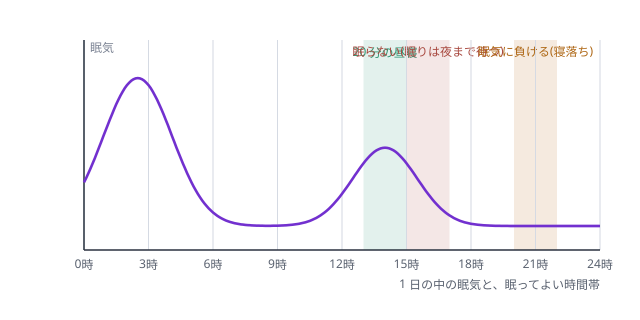
\includegraphics[width=0.8\textwidth]{figures/nap-map.svg}
\caption{1 日の中の眠気と、眠ってよい時間帯。午後の早い時間帯は眠気が高く、かつ夜への悪影響が少ない。20 時以降は夜に響くため避ける。}
\end{figure}

\subsection{カフェインナップ}

\textbf{「カフェインナップ」}という方法があります。\textbf{カフェインを飲んですぐ 20 分眠る}、という順序です。
その理由は、\textbf{カフェインが血液中に届くまでに 20 分ほどかかる}ためである。\textbf{ちょうど眠りについた頃にカフェインが効き始める}ため、\textbf{目覚めたときに目が覚める}。

\begin{quote}
\textbf{【演習】}\ 13 時に 20 分寝る場合と、14 時に 20 分寝る場合を比べよ。\textbf{考慮すべき要素}は何か。
\end{quote}

\textbf{解答の指針:}\ どちらも 20 分なら夜の入眠への影響は小さい。\textbf{午後 1 時が概日リズムの谷の中心に近く、効果が高い}。\textbf{15 時を過ぎると谷を過ぎるため効果が減り}、かつ午後 3 時以降はカフェインのタイミングともかぶります。\textbf{「13 時から 15 時」の間が最も安全}といえます。

\section{睡眠の問題と支援の受け口}

睡眠の問題は、「頑張れば消える」ものではありません。\textbf{典型的な症状と、それぞれの相談先}をまとめます。

\subsection{いびきと無呼吸}

いびきは、空気の通り道が狭くなるときの音です。\textbf{いびき中高に息が止まる}場合は、\textbf{閉塞性睡眠時無呼吸(OSA)}の可能性があります。

OSA の典型的な特徴は、いびきが繰り返されること、\textbf{寝ている間に息が止まること}、日中の強い眠気、\textbf{朝の集中力の低下}です。\textbf{OSA は了自己努力で治るものではありません}。\textbf{医療機関での相談が必要です}。

\subsection{不眠と「眠れないことへの心配」}

不眠は、\textbf{入睡困難}(寝つけない)、\textbf{中途覚醒}(途中で目覚める)、\textbf{早番覚醒}(早すぎる)に分かれます。

\textbf{眠れないことを恐れている場合}、\textbf{妙な悪循環}が生まれます。\textbf{眠ろうとするほど眠れない}。\textbf{「眠れることへの執着」が、眠ることそのものの障害になる}。\textbf{覚醒を避けること}が逆に眠気を強めます。

\subsection{脚のむずむず}

\textbf{脚に落ち着かない感覚}があり、\textbf{動かさないと落ち着かない}。\textbf{就寝前や夜中に悪化}することが多い。\textbf{鉄分の不足}と関係があるとされています。

\subsection{概日リズム睡眠障害}

体内時計の位相が大きくずれている状態です。\textbf{「普通の時刻に眠れない」}のが特徴です。
寝たい時刻が早すぎる場合と、遅すぎる場合があります。\textbf{時差(jet lag)}も、体内時計のずれの軽い現象です。

\begin{quote}
\textbf{【演習】}\ 2 週間毎日午前 2 時に寝て午前 11 時に起きている学生がいます。\textbf{この学生の睡眠は「質が悪い」のか、「タイミングが違う」だけか}。\textbf{判断の材料}を 2 プロセスモデルから述べよ。
\end{quote}

\textbf{解答の指針:}\ 睡眠段階の構成には問題がない。\textbf{2 プロセスモデルで言えば、S と C のタイミングだけが合っていない}。\textbf{これは「質の問題」ではなく「体内時計の問題」です}。\textbf{数週間続くなら、医療機関で相談してください}。

\section{性能への効果 — 記憶、判断、そして免疫}

ここまでは「睡眠とは何か」でした。\textbf{ここからは「睡眠をすると何が変わるか」}を検証します。

\subsection{記憶の定着}

試験前夜に勉強した内容は、翌朝に思い出せますか。\textbf{答えは、眠ったかどうかで変わります}。

\begin{quote}
\textbf{【例:効果量の大きさ】}\ 2024 年のメタ分析の 1 つでは、\textbf{睡眠制限が記憶の符号化に及ぼす効果量が 0.4 程度}と報告されています。\textbf{ただし、対象は健康的な若者に限定されており、長期間の睡眠制限への外挿は不確か}です。
\end{quote}

\begin{quote}
\textbf{【演習】}\ 記憶の効果量が \textbf{0.4} であったという報告を受けて、「\textbf{睡眠は記憶を 1.4 倍にする}」と説明した場合、何が間違っているか。
\end{quote}

\textbf{解答の指針:}\ 効果量 \(d = 0.4\) は、\textbf{「標準偏差 0.4 個分の差」}にすぎません。\textbf{「1.4 倍」という表現は正しくありません}。\textbf{比の表現は基準値に依存するため、統計的には効果量と信頼区間で語るべき}です。

\subsection{判断力と創造性}

一夜の睡眠制限で、\textbf{判断の誤りは増える}ことが報告されています。

\textbf{8 時間に対して 5 時間では、反応時間が 20〜30\% 劣る}、という報告があります。\textbf{まだ「眠れない」ほどではないとしても、「軽微な眠気」は同じ程度の損失}です。

\section{今週の睡眠改善計画}

ここまでの各節から、「何を変えればよいか」が具体的に決まりました。\textbf{ただし全部を一度にやろうとしないこと}。本章は、\textbf{来週 1 週間だけ続ける 3 つ}を選ぶための基準と、実際の記録の書き方を示します。

\subsection{3 つだけ選んで 1 週間}

本書は 10 以上の方法を説明しました。しかし全部を同時にやろうとすると、\textbf{毎日に何をしたかを確認する手間が増え、3 日目には止まる}ことがあります。睡眠の改善は、\textbf{1 回に入れられる変更の量より、その変更を続ける期間}のほうが結果を左右します。

\begin{quote}
\textbf{【要点】}\ \ 1 週間の計画は 3 項目まで。4 つ以上を同時に始めると、どれが効いたか分からなくなり、\textbf{4 つともやめてしまう}結果になります。3 つなら、\textbf{毎日に何をするかを考え直さずに済む}ため、1 週間保つことができます。
\end{quote}
選んだ 3 つに共通するのは、\textbf{効果が大きい反面、その日のたびに迷わない}ことです。どれか 1 つを選べず、\textbf{どれをやるか毎回考えている状態では変更は続きません}。
\begin{enumerate}
\item \textbf{起きる時刻を毎日固定する}: 平日と休日で、起床時刻の差を 1 時間以内に収めます。第 7 節の式に従うと、\textbf{起きる時間を決めれば入眠時刻は結果として決まる}ため、最初に決める数字は就寝時刻ではなく起床時刻です。
\item \textbf{朝の 10 分を屋外で過ごす}: 目が覚めてから 10 分以内に外に出ます。屋内の照明はおよそ 100〜500 ルクス、屋外は 10 万ルクス以上なので、\textbf{外に出ること自体が光の量を変えます}。午後ではなく、\textbf{朝起きてすぐの 10 分}に行うのが要点です。
\item \textbf{午後 3 時以降のカフェインをやめる}: 半減期 5.5 時間で、午後 3 時に 200 mg を飲むと翌朝 6 時の 15 時間後にはおよそ 1/8 が残ります。\textbf{入眠時刻を遅らせる理由は、飲んだ量ではなく飲んだ時刻にある}からです。
\end{enumerate}
3 つを 1 週間だけ試したあと、\textbf{続けられないものを 1 つだけ外します}。残した 2 つを次の 1 週に持ち越します。\textbf{最初から全部を同時に始めない}ことが、1 週間より長い期間まで続けるための要点です。

\subsection{Epworth の眠気の尺度}

日中の眠気を測る方法に、\textbf{Epworth の尺度}があります。\emph{はい / いいえ} の 8 問で、\textbf{日中の眠気が生じた場面を数える}方式です。\textbf{眠気の程度を聞くのではなく場面で確認する}ので、その日の気分ではなく\textbf{1 か月間}の発生頻度が得られます。
最近 1 か月の通常の暮らしについて、次の 8 問に答えます。\textbf{眠気の程度ではなく、場面ごとの発生頻度}を数える点が要点です。
\begin{enumerate}
\item 読書中のとき、ときどき眠くなる。
\item 集会や講演のときに、ときどき眠ることがある。
\item 席に座っているだけのとき、ときどき眠くなる。
\item 車の運転席で止まっているとき、ときどき眠くなる。
\item 電話中で、ときどき眠くなる。
\item 休憩中やひまの時間に、ときどき眠くなる。
\item 午後、落ち着かないときに、ときどき眠気を感じる。
\item 眠いまま、人を乗せて車を走らせているとき、ときどき眠くなる。
\end{enumerate}
得点は \textbf{0〜24 点}です。\textbf{11 点以上で日中の眠気が強い}という目安が使われることがあります。\emph{ただし、これはスクリーニングであり、診断ではありません}。点数だけで原因を決めつけず、\textbf{医療機関で確認する材料の 1 つ}にすぎません。
\subsection{1 週間の記録表}

3 つの変更を続けるときは、\textbf{就寝時刻と起床時刻、そして日中の眠気を毎日 1 行}で記録します。\textbf{記録は 1 行で足りる}ため、\textbf{記録そのものが負担になりにくい}大きさです。
\begin{center}
\begin{tabular}{|c|c|c|c|}
\hline
日 & 就寝時刻 & 起床時刻 & 眠気(0〜10) \\
\hline
1 & 23:00 & 7:00 & 3 \\
\hline
2 & 23:00 & 7:00 & 3 \\
3 & 23:00 & 7:00 & 3 \\
\hline
4 & 23:00 & 7:00 & 3 \\
5 & 23:00 & 7:00 & 3 \\
\hline
6 & 23:00 & 7:00 & 3 \\
7 & 23:00 & 7:00 & 3 \\
\hline
\end{tabular}
\end{center}
眠気は 0(眠くない)から 10(眠くて動けない)までを、その日のあとで記入します。\textbf{毎日細かく書き込む必要はありません}。\textbf{1 週間に 1 回だけ記入すれば十分}です。\textbf{記録すること自体が負担になっては、計画は続きません}。
この表は、\textbf{3 つの変更が 1 週間で保てたかを確かめる道具}です。\textbf{自分の行動を記録するものであって、医療上の判断には使いません}。\textbf{点数が高ければ重い、という意味ではありません}。

\section{総合演習}

ここまでの各節から、要点を選びました。\textbf{12 問}すべてが、本文の数値と矛盾しないことを確かめてください。

\begin{quote}
\textbf{【演習 1】}\ カフェインの半減期は 5.5 時間である。\textbf{午後 3 時に飲んだカフェインが、翌朝 6 時(15 時間後)に何\%残るか}を求めよ。
\end{quote}

\textbf{解答の指針:}\ 15 時間は半減期 5.5 時間の \(15 / 5.5 \approx 2.73\) 倍である。\textbf{残る割合は \((1/2)^{2.73} \approx 0.15\)}、\textbf{およそ 15\%(概算で 1/7 程度)}である。本書では 3 回の半減期にあたるとして 1/8 と概算している。\textbf{半分は消えていても、半分は残っている}。重要なのは\textbf{飲んだ量ではなく飲んだ時刻}である。

\begin{quote}
\textbf{【演習 2】}\ カフェインの半減期は 5.5 時間である。\textbf{午前 9 時に飲んだカフェインが、正午(3 時間後)に何\%残るか}を求めよ。
\end{quote}

\textbf{解答の指針:}\ 3 時間は半減期の \(3 / 5.5 \approx 0.55\) 倍なので、\textbf{残る割合は \((1/2)^{0.55} \approx 0.69\)}、\textbf{およそ 69\%(概算で 7 割)}である。演習 1 と合わせて読むと、\textbf{減り方が早いのでなく、同じ割合で減り続ける}ことが分かります。\textbf{1 時間あたりの減少幅を足し算で求めるのは誤り}です。

\begin{quote}
\textbf{【演習 3】}\ ある人が Epworth の尺度で 12 点を取った。\textbf{この解釈として正しいものは何か}。ただしこの尺度はスクリーニングであり、診断ではない。
\end{quote}

\textbf{解答の指針:}\ 正しいのは、\textbf{日中の眠気が強いという状態の目安}を示したものであることである。\textbf{11 点以上が目安}とされるので、12 点はそれを上回る。\textbf{しかしこれはスクリーニングであり診断ではない}。\textbf{原因が何か、病名が付くかをこの点数で決めてはならず}、\textbf{医療機関で確認する材料の 1 つ}として扱う。

\begin{quote}
\textbf{【演習 4】}\ 「1 サイクルは 90 分」という言い回しが不正確である理由を述べよ。\textbf{一晩の睡眠では、深い睡眠と REM の配分が均等に繰り返されない}ことを根拠にすること。
\end{quote}

\textbf{解答の指針:}\ サイクルの幅は\textbf{人によって異なり、その夜のなかでも変動する}。\textbf{N3 は前半に偏り、REM は後半に向かって伸びる}ため、\textbf{同じ幅の山が等間隔で続くという前提が成り立たない}。90 分は平均値にすぎず、\textbf{90 分ちょうどを起こそうとすると、最も深い睡眠の途中か REM の途中で起きることになる}。\textbf{起きる時間はサイクルと関係なく、総睡眠時間だけで決める}。

\begin{quote}
\textbf{【演習 5】}\ プロセス S(睡眠圧)とプロセス C(覚醒推進)は、それぞれ\textbf{いつ低下するか}。\textbf{この 2 つの時間的な違いが、昼寝の説明にどう使われるか}述べよ。
\end{quote}

\textbf{解答の指針:}\ \textbf{プロセス S は眠ると同時に下がり、眠っているあいだに作用する}のに対し、\textbf{プロセス C は概日リズムに支配されているので、昼寝では下がらない}。\textbf{体内時計は「まだ昼だ」と認識している}からである。\textbf{そのため 20 分なら夜への影響は小さいが、1 時間以上は翌夜の入眠を遅らせる}。

\begin{quote}
\textbf{【演習 6】}\ 1 晩だけの不足と、数週間続く不足では意味がどう違うか。\textbf{睡眠負債の回復に何晩かかるか}という具体を示して述べよ。
\end{quote}

\textbf{解答の指針:}\ \textbf{回復には 2 晩ほどかかる}ので、\textbf{1 晩だけの不足は 2 晩の通常の睡眠で元に戻せる}。一方、\textbf{週に 6 日 4 時間しか眠らない場合、負債は蓄積する一方で回復が追いつかない}。\textbf{取り戻そうとして昼寝を長くすると、体内時計がずれ、次の夜に入れなくなる}。\textbf{悪い夜の翌朝は平时どおりに起きること}が正解である。

\begin{quote}
\textbf{【演習 7】}\ 閉塞性睡眠時無呼吸(OSA)の典型的な特徴を 3 つ挙げよ。\textbf{さらに、どちらの機関に相談すべきかも述べよ}。
\end{quote}

\textbf{解答の指針:}\ \textbf{① 大きないびき、② 寝ているあいだに息が止まる、③ 日中の強い眠気}の 3 つである。\textbf{朝の集中力の低下}も添えよう。\textbf{OSA は自分で努力しても治るものではない}ため、\textbf{医療機関での相談が必要}である。\textbf{「閉塞性睡眠時無呼吸」と書く}ことで、\textbf{空気の通り道が詰まる型の無呼吸}であることを示す。

\begin{quote}
\textbf{【演習 8】}\ 20 分の昼寝と 90 分の昼寝の違いを述べよ。\textbf{90 分の場合はどのような悪い結果が起こりうるか}も述べよ。
\end{quote}

\textbf{解答の指針:}\ 20 分は\textbf{深い睡眠に入るか入らないかの境界}にあたり、\textbf{睡眠酔いの副作用が最小}で済む。90 分は 1 サイクルをまるごと含むため、\textbf{REM に入るので、起床直後に深い眠気(睡眠酔い)が出る}。\textbf{その眠気が取れずに次の行動へ移ると、パフォーマンスが落ちる}。\textbf{午後 1 時から 3 時の 20 分が、安全と効果の両方がそろった位置}である。

\begin{quote}
\textbf{【演習 9】}\ アルコールを飲んでから寝たとき、REM 睡眠はどう変化するか。\textbf{入眠が早いのに翌朝の気分が悪いのはなぜか}述べよ。
\end{quote}

\textbf{解答の指針:}\ \textbf{アルコールは REM 睡眠を著しく削り}、\textbf{代謝が進むにつれ後半の覚醒が増える}。\textbf{REM を一度抑えた後、その反動で REM が通常より多く出る現象を反動(rebound)と呼ぶ}。\textbf{入眠は早いが途中の質が崩れる}ので、\textbf{「よく眠った」と感じない}。\textbf{翌朝すっきりしないのは、深い睡眠が取れた証拠ではなく、後半が断片化しているため}である。

\begin{quote}
\textbf{【演習 10】}\ 起床時刻を毎日 30 分ずつ早める計画を継続した場合、\textbf{体内時計とのずれが積み上がるか}述べよ。\textbf{その計画が失敗する条件を}、社会時差の観点から説明せよ。
\end{quote}

\textbf{解答の指針:}\ \textbf{体内時計はおよそ 24.2 時間の周期}で回っているため、\textbf{毎日 30 分だけ早めると、ずれがそのまま積み上がる}。\textbf{時差と同じ現象}である。\textbf{眠れない夜が続いたときは、起床時刻を早めるのではなく平时にもどす}。\textbf{体内時計が動くには数日を要するため、短い期間での結論は出せない}。

\begin{quote}
\textbf{【演習 11】}\ 朝の屋外で 10 分の光を受けることが、体内時計にどう働くのか、\textbf{最も近い説明は何か}。
\end{quote}

\textbf{解答の指針:}\ \textbf{朝の光は体内時計の位相を早める方向に動かす}。\textbf{夕方の光は逆方向に動かす}。\textbf{消灯時刻ではなく起床時刻を揃えるべきな}のは、\textbf{この方向の差が理由}である。\textbf{屋内の 100〜500 ルクスでは、屋外の 10 万ルクス以上と効果が違う}ため、\textbf{時間だけでなく光の量も設計の対象}になる。

\begin{quote}
\textbf{【演習 12】}\ 「眠れない」ことと「眠れないのが怖い」ことはどう違うか。\textbf{眠れないことへの心配が長期に続く場合に使う用語は何か}。
\end{quote}

\textbf{解答の指針:}\ \textbf{眠れないこと}は寝つけない、途中で起きるなど、\textbf{睡眠の状態そのものの問題}である。一方、\textbf{眠れないのが怖い}ことは、\textbf{眠ろうとするほど眠れなくなる状態}を指す。\textbf{覚醒を避けること}が逆に眠気を強くする。\textbf{この心配が長く続くものを不眠恐怖症と呼ぶ}。\textbf{数週間続くなら、医療機関で相談する}。

\begin{quote}
\begin{quote}
\textbf{【心構え】}\ \textbf{睡眠は与えられるものではない}。\textbf{設計できる}。起床時刻を固定する、\textbf{朝に光を受ける}、\textbf{午後 3 時以降のカフェインをやめる}——この 3 つに改善の多くがある。\textbf{一方で、設計では解決しない問題が残る}。不眠、\textbf{無呼吸}、\textbf{定期的な強い昼間の眠気}は、\emph{医療機関に相談する}。\textbf{本書は一般的な情報であり、医療上の助言ではありません}。
\end{quote}
\end{quote}

\end{document}
